\begin{MyChapter}{Játékfejlesztés általánosan}
	% TODO 	- mi lesz a fejezetben

	\begin{MySection}{Játékfejlesztés történelme}
		% honnan indult a játékfejlesztés 
		% fontosabb játékok megemlíteni
		% fejlődési mérföldkövek (új effektek, megjelenítés, fizika stb, mi mikortól jelent meg, esetleg mire/miért jó)
		
		A játékfejlesztés történelme egészen az 1950-es évekre nyúlik vissza, amikor már egyes informatikusok az egyetemeken elkezdtek egyszerűbb játékokat, valamint szimulációkat készíteni a kutatásaik egy részeként, azonban ezek nem lettek bemutatva a nyilvánosságnak, nem voltak elérhetőek mindenki számára.  \cite{video_game_development}
		
		Az első videojátékok közé sorolhatjuk a "Tennis for Two"-t, amelyet William Higinbotham amerikai fizikus készített egy Donner Model 30 típusú analóg számítógépre. Ez egy oldalnézetes asztalitenisz szimulátor volt, az első olyan játék, amely grafikus kijelzőt használt.
		Ide sorolható még például a Sandy Douglas brit informatikus által fejlesztett "OXO", amelyben a 3x3 darab mezőbe a számítógép és egy játékos felváltva teszik a szimbólumokat, mindaddig, amíg valamelyiküknek nem sikerül 3 darab egy vonalban álló mezőbe azonos szimbólumokat tenni. Ez tulajdonképpen a "Tic-tac-toe" játéknak egy korábbi alternatívája, 1952-ből.
		Hasonlóan az előzőekhez, a "Spacewar!" nevű játék is az első játékok közé tehető, amit 1962-ben az MIT-n (Massachusetts Institute of Technology) Stephen Russel amerikai informatikus néhány diáktársával együtt alkotott. A Spacewar! két játékos között szimulált egy űrbéli harcot. 
		
		% TODO Tennis for Two / OXO / Spacewar! fotó(k)??
		
		\begin{MySubSection}{Első publikus játékok}
		Egészen az 1970-es évekig még nem értek el nagy népszerűséget a videojátékok, csak ekkor kezdtek el olyan játékokat fejleszteni, amiket a nyilvánosság számára is elérhetővé tettek. Ekkor kezdték el árulni a konzolok első generációját is, például a Magnavox Odyssey-t, valamint a Color TV-Game-t. Ezek a televízión való játszást tették lehetővé a felhasználók számára, otthon.
		
		Az első konzol prototípusát "The Brown Box" (magyarul: a barna doboz) névre keresztelték el, ez lett a későbbiekben, 1972-ben kiadott Magnavox Odyssey. Ennek a grafikája fehér pontokból és vonalakból állt. A játékoknak nem volt háttérgrafikájuk, hanem a rendszer 2 különböző méretű (nagy és közepes), áttetsző képernyő átfedéskészletet(Overlay% TODO overlay fordítás (?) https://www.lifewire.com/magnavox-odyssey-the-first-gaming-console-729587 -> Graphics and Screen Overlays
		) használt. Néhány játék számára nem volt szükség háttérre, míg más játékoknál kötelező volt. Tartalmazott többek között foci, kísértetház, tenisz, hoki, és egyéb átfedéseket. Itt még nem volt memória amibe eltárolhatta volna a pontszámokat a konzol, így külön ponttáblát kellett hozzá használni, illetve játékkártyákat, melyek behelyezésével indult el a rendszer. Például a "Football" játék két cartridge-re volt szétosztva. A cartridgek egy nyomtatott áramkörből állnak, melyet műanyag borítás védelmez, egy csatlakozón keresztül kommunikál a konzollal. Ezek tulajdonképpen az első külső memóriák voltak, melyeket a házi konzolokhoz használtak. A kettőből az egyik a futás, a másik pedig a passzolás, rúgás volt. Mivel nem rendelkezett mentés funkcióval a konzol, a használónak kellett számon tartania a pontot és a pozíciókat a Magnavox Odyssey-hoz tartozó pont- és játékkártyákkal, a két cartridge cserélgetése közben. Viszont ezeket a kiegészítőket gyakran elhagyták a használók, így manapság már egy komplett Magnavox Odyssey rendszert szinte lehetetlen lenne találni. A konzol egyik játéka adott egyébként inpsirációt az egyik első árkád játéknak, a "Pong"-nak, ami játéktermekben volt fellelhető 1972-től, célja pedig, hogy a labdát játékban tartsuk, ezzel növelve a pontjaink számát. Mára a Pong már kifejezetten népszerű lett, sok másolata, klónja is készült a sikeressége miatt, illetve több platformra is átkerült.
		
		% TODO kép az első konzolról(?) / Pongról
		
		Körülbelül ekkor kezdtek el hatalmas népszerűségre szert tenni az árkád játékok. Különösképpen a "Space Invaders" kiadása után, 1978-ban volt ez megfigyelhető, ami egy egyszerű, mégis addiktív és adrenalindús játék volt, melynek célja, hogy a játékos megmentse a Földet az alien-ektől. Érdekesség, hogy eredetileg sokkal lassabb játékmenetet tervezett a készítője, azonban problémába ütközött az állandó tempó megtartásában, így végül folyamatosan növekszik a sebesség, egyre nehezítve a játékmenetet, a játékosok pedig pont így szerették meg a játékot. Az árkád játékok közül még érdemes megemlíteni a "Pac-Man"-t, mely szintén nagyon közkedvelt lett.

		% TODO arcade games kép?
		
		Szintén az 1970-es évek végén egyes étteremláncok elkezdtek videojáték gépeket betelepíteni üzleteikbe, ez tulajdonképpen a többszereplős játékok gyökere volt. Ez akkoriban azt jelentette, hogy akik ugyanazon a gépen játszottak, a többi játékos pontszámát láthatták a toplistán, így tudtak versenyezni egymással. Az online többszereplős játékok csak később kaptak helyet a szórakoztatóiparban.
		
		A PC játékok első generációjánál gyakoriak voltak a szöveg alapú kalandjátékok, amelyekben a játékosok billentyűzeten keresztüli rövid parancsok által tudták irányítani a játékmenetet. Egyik legfontosabb ilyen játék például a "Colossal Cave Adventure", melyet Will Crowther, barlangász és programozó alkotott 1976-ban, egy évvel később pedig Don Woods segítségével kibővült a játék. A kalandjátékban egy rejtélyes barlangot fedezhet fel a játékos, melyben aranyat, kincset találhat, a cél pedig minél több pontot gyűjtve, élve kijutni a barlangból.
		1979-ben alakult meg az Activision cég, mely egy fontos mérföldkő a játékfejlesztés történelmében, tekintve, hogy ez volt az első független videojáték fejlesztő és kereskedő. A korai 1980-as években számos sikeres játékot adtak el. Terveztek jó néhány meghatározó és emlékezetes játéktapasztalatot adó játékot a felhaszálók számára.
		Szintén ekkor, játékmagazinok és hobbiból programozók által jött létre és került nyilvánosságra rengeteg játék, mivel otthon is viszonylag könnyen lehetett ekkor leprogramozni egy játékot. Ezekhez a forráskódot is mellékelték, ezáltal kedvükre módosíthatták azt a játékosok. Fontosabb játék volt ekkoriban a "Microchess", mely az egyik első olyan játék volt, amit mikroszámítógépekre gyártottak.
		\end{MySubSection}
		
		\begin{MySubSection}{1983-mas videojáték krízis}
		Egyre többen szerettek volna bevételt szerezni a videojátékokból, a konzolok ára csökkent, az igény az új játékokra nőtt, a fejlesztők nem győztek eleget tenni a követelményeknek. A piac telített volt a konzolok terén az átlag fogyasztót összezavarva ezzel, hogy vajon melyiket is válassza. A konzolok bősége miatt kevéssé vált lehetővé a barátokkal való játék is, ha megveszel egy drága konzolt majd mindegyik barátod másfajtát vesz, kevésbé lesz élvezetes a játék. Ezenkívül a konzolgyártók kezeiből kicsúszott az irányítás a platformjaikra gyártott játékok terén. A játékpiac tele volt gyenge minőségű játékokkal is, melyek még nem álltak készen az eladásra, így hiába volt néhány remek játék mert a rengeteg rossz játék miatt a cégek bevétele apadni kezdett. Jétékok milliói sosem lettek eladva, annyira szörnyűek voltak, így rengeteg el lett ásva Új Mexikóban. Mindeközben az otthoni számítógépek ára csökkent, hasonló áron lehetett hozájutni, mint egy konzolhoz, emiatt szokásossá váltak az otthoni számítógépek. Egy számítógép új és fejlettebb platformot nyújtott a játékoknak, emellett pedig más funkciókat is betöltött, nem úgy mint egy konzol, ezzel jelentősen csökkentette a fogyasztói érdeklődést az árkád játékokra és a konzolokra. 1983 végére többek között az előbbi tényezők hatására, nagy gazdasági visszaesés történt, a kritikusok úgy ítélték meg, hogy a videojátékoknak annyi, jó néhány videojátékgyártó cég csődbe ment, vagy szimplán nem gyártott több játékot.
		A számítógépes játékok viszont így lényegesen előtérbe kerültek.
		\end{MySubSection}
	
		\begin{MySubSection}{A videojáték-piac újjászületése}
		Azonban fontos megemlíteni a Nintendo vállalkozást, amely a piac összeomlásának következtében méginkább helyet kapott a videojátékpiacon. A cég az 1970-es évek végén kezdett érdeklődni a videojáték-piac iránt. Érdekesség, hogy azelőtt az 1889-ben alakuló cég hanafudának nevezett kártyajátékokat gyártott illetve értékesített. 1956 és 1975 között több üzletágban is kipróbálták magukat, azonban végül a videojáték gyártás lett a fő profilja. Kiemelendő a "Donkey Kong", mely egyik leghíresebb játéktermi játéka volt a Nintendo-nak. 1981-ben alkották meg, és a világ ebben a játékban ismerhette meg először Mario karakterét, aki a későbbiekben a "Mario Bros." valamint a még későbbi "Super Mario Bros." egyik főszereplőjeként tűnt fel. A Nintendo kipróbálta magát a kézi konzolok gyártásában is, 1985-ben adta ki a NES-nek nevezett gépét (Nintendo Entertainment System), mellyel szintén nagy sikereket ért el. A NES-nél kifejezetten odafigyeltek a magas minőségű játékokra, és sikerült visszanyerniük a fogyasztók bizalmát. Következő óriási sikerét 1989-ben érte el, a Game Boy kiadásával, mely egy 8 bites kézi videojáték-konzol volt. 1990-ben pedig kiadta a SNES-t (Super Nintendo Entertainment System), dominálva ezzel a játékpiacot. Még kazettákat kellett hozzá használni, viszont grafikus képességeivel, a játékok kinézetével, és a hanggal, ez a készülék áthidalja a régi videojátékok és a modern korszak közötti szakadékot. A cég hatalmas hírnevet szerzett magának az utóbbi termékvonalainak fejlesztésével, frissítésével, fokozatosan elérve, hogy napjainkig a világ egyik legismertebb videojáték-gyártója váljon belőle. %Érdekességként megfigyelhetjük 1997-től a Nintendo által gyártott otthoni konzolokat egészen 2020-as évig. (lásd: \myref{fig:nintendos-unit-sales-of-video-game-consoles-1997-2020} ábra)
		
		% TODO ez a link esetleg érdekességként? (+ ezelőtti mondatot kikommentezni ha kell)
		% https://www.statista.com/statistics/227012/lifetime-unit-sales-of-nintendos-home-consoles/
		%
		%\begin{figure}[h!]
		%	\centering
		%	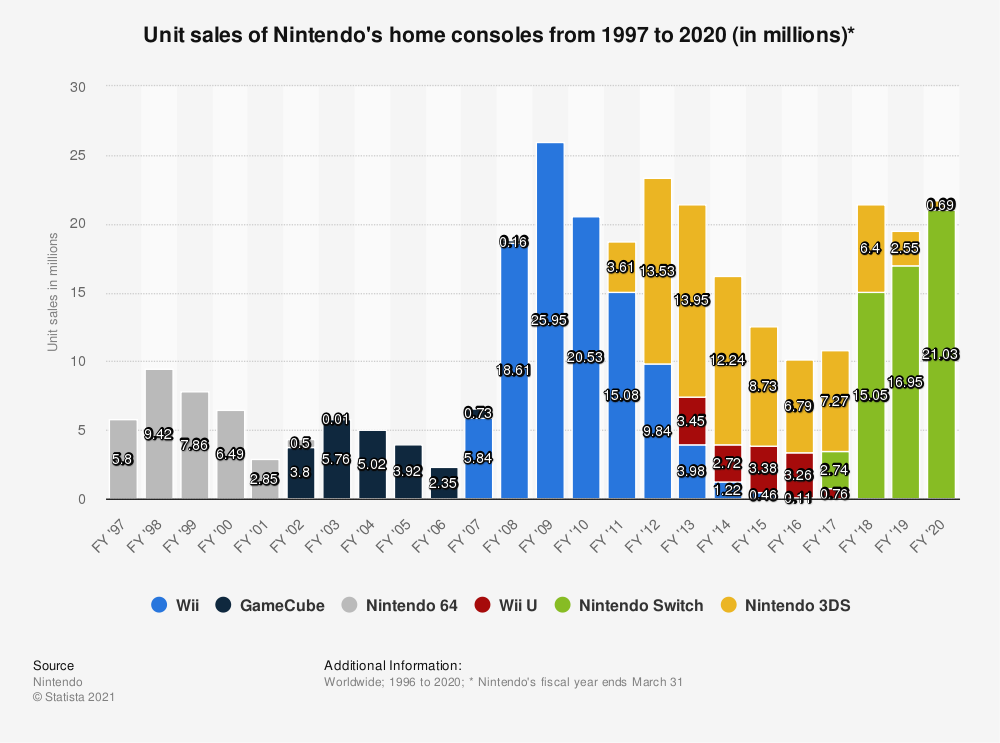
\includegraphics[scale=0.38]{kepek/nintendos-unit-sales-of-video-game-consoles-1997-2020.png}
		%	\caption{Nintendo otthoni konzolainak eladási statisztikája 1997-2020-ig}
		%	\label{fig:nintendos-unit-sales-of-video-game-consoles-1997-2020}
		%\end{figure}
		
		Másrészről, a Sony kifejlesztette 1994-ben az első CD-alapú konzolt, a PlayStation-t, mely erősségei közé sorolhatjuk a 3 dimenziós grafikát, valamint a CD-ROM technológia által adott hang- és képminőséget. A konzol képes volt nem csak a játékok futtatására, hanem emellett audio CD-k lejátszására is. A PlayStation-nel már szándékosan nem csak a gyerekeket, hanem a felnőttebb korosztályt is megcélozta a Sony, ebben az időszakban kezdett hétköznapivá válni idősebbek körében is ez a fajta szórakozási lehetőség. A PlayStation által ismerhettük meg a "Final Fantasy"-t, a "Tekken"-t, vagy épp a "Silent Hill"-t, melyek a mai napig ismert névnek számítanak.
		
		A PlayStation 2000-ben kiadta utódját, a 6. generációs konzolt, PlayStation 2 névvel (röviden: PS2), amely meglehetősen gyorsan népszerűvé vált. Több exkluzív név köthető hozzá, mely más platformon nem jelent meg. Egészen 2013-ig népszerű maradt, és folytatódott a gyártása, pedig akkorra már az utána következő PlayStation 3 is megjelent. A PS2 még napjainkban is a világ legnagyobb darabszámban értékesített konzolja.
		
		\end{MySubSection}
		
		\begin{MySubSection}{A videojátékok további fejlődése}
		Korábban volt szó, az online játékokról, ennek elérésével többször próbálkoztak a fejlesztők, viszont hosszú ideig sikertelenül. Az első igazán népszerű online szerepjáték az 1997-es Massively Multiplayer Online Role-Playing Game (röviden: MMORPG) az Ultima Online volt, chat funkcióval, lehetővé téve a játékosok közötti interakciót és kommunikációt. Konzolok terén 2000-ben a Sega Dreamcast megjelentette első internetre-kész konzolját, egy igazán forradalmi rendszert, és az első internetes eszközt ami népszerűséget is szerzett. Azonban még ez is bukásra volt ítélve, tekintve, hogy még ekkor is kifejezetten költséges volt az internethozzáférés, így a Sega a felhasználók általi játék után hatalmas összegű számlákat kapott. A Sega kudarcának következtében a konkurens konzol-gyártók tanultak a negatívumokból, és a fejlesztéseiknek köszönhetően a 2000 körüli években az online funkcionalitás már nélkülözhetetlenné vált a játékiparban.
		
		A hardvergyártók egyre inkább felismerték a rengeteg potenciális üzleti lehetőséget, amik a multimédiás alkalmazásokban, videojátékokban rejlettek, rájöttek, hogy ezeken a területeken nagyobb teljesítményű hardverekre volt igény.
		A CPU (processzor) gyártók 2005 körülre már egyenesen a több magos processzorok felé haladtak. 
		GPU (videokártya) terén, az NVidia 1995 májusában jelentette be első grafikus kártyáját, az NV1-et, az ATI pedig szintén abban az évben, novemberben adta ki első 3D-s gyorsító kártyáját, a 3D Rage-et. Még azonban rengeteg problémával kellett megküzdeniük a gyártóknak. Az ATI 3D Rage végső változata, az ATI Rage 128 volt amely 1999-ben teljesedett ki. Ugyancsak 1999-ben látott napvilágot az NVidia GeForce 256 (avagy más néven NV10), amellyel az NVidia átvette a vezető szerepet a teljesítmény-versenyben.
		
		Ezt megelőzően, amikor a számítógépek még nem tartalmaztak speciális, grafikai számítások gyorsítására használt feldolgozó egységet, még minden számítási feladatot a CPU végzett. Ezt a korai megjelenítési formát szoftveres raszterizációnak nevezzük. Ezzel a módszerrel tulajdonképpen a programozó teljes mértékben képes volt kezelni a megjelenítési folyamatokat, ami elég nagy rugalmasságot jelentett.
		Azonban a szoftveres raszterizáció hátránya, hogy nagyobb adathalmaz mozgatása és kezelése lassabban kivitelezhető a módszerrel, mint a grafikai processzorokkal.
		Ez azért fontos, mert a számítógépes grafikában lényeges célkitűzés volt a részletes, valósághű ábrázolás elérése, ami viszont nagy energiaforrásigényű, így a textúra szűréseket nem alkalmazó szoftveres megjelenítés, kimondottan egy 3D játék esetén lényeges eltérést mutatott már az első GPU-khoz képest is. \cite{mileff}
		% TODO irodalom -> 
		% https://users.iit.uni-miskolc.hu/~mileff/grafika/Grafika_programozasa_jegyzet_v0.66_Mileff_P.pdf
		
		A grafikai protesszorok megjelenése után, melyek tehát a valósidejű komplex kép kirajzolását gyorsítják, nagy lökést kapott a játékipar. Egyre inkább előtérbe kerültek a 3D-s játékok, mivel már volt lehetőség jobb minőségben elkészíteni őket, illetve a videokártya könnyen hozzáférhető volt és megfizethető, ezáltal gond nélkül elterjedt, a 3D-s játékok népszerűsége pedig azóta is töretlen.
		A hardvergyártás fejlődésének köszönhetően a videojátékok egyre filmszerűbbek és komplexebbek lettek, egyre inkább eladhatóvá váltak. Vegyük például a korábban említett Silent Hill-t, melynek atmoszféráját, a hangeffekteket, a grafikát kifejezetten eltalálta a PlayStation. Mindezek nélkül, más rendszerben, környezetben nem állta volna meg a helyét ennyire sikeresen ez a játék.
		
		A korábbi, hobbiból programozott játékok helyett jelentősen megnőtt az igény a modernebb, magasabb színvonalú játékfejlesztésre. 
		Így tehát a számítástechnika fejlődésével és az internet adottságainak jókora megnövekedésével, illetve elterjedésével egyre inkább jelentős részévé váltak a játékok a szórakoztatóiparnak, az előző generációt teljesen elsöpörve a fedélzetről.
		\end{MySubSection}
				
	\end{MySection}

	\begin{MySection}{Játékfejlesztés alapjai} 
		% TODO 	- játékfejlesztés alapjai ?
		% TODO 	- játékfejlesztés menete ?
		% pc
		
		\begin{MySubSection}{PC játékok}
			Fentebb már szó volt róla, hogy a számítógépes játékok az 1983-mas videojáték válság idején sokkal elterjedtebbé váltak, mint az egyéb platformokon lévők. 1984-re a számítógépes játékok vették át a vezetést a játék-piacon a konzolok helyett.
			A csúcskategóriás PC-játékok szempontjából kifejezetten fontos, hogy a számítógépek általában sokkal több erőforrásssal rendelkeznek mint más játékrendszerek, platformok. A játékfejlesztők számára a jobb hardver lehetővé teszi a játékaik realisztikusabb és részletgazdagabb elkészítését a többi platformhoz viszonyítva. Itt gondolhatunk például részletesebb grafikai elemekre, melyet a nagyobb számítási kapacitás tesz lehetővé, vagy a gazdagabb felhasználói felületre, melyet a nagyobb felbontású megjelenítők, illetve a precízebben mozgatható egér használata tesz lehetővé. A felhasználói felületetes példánál maradva, egy konzolra nem érdemes olyan kezelőfelületet csinálni aminek sok menüpontja van, hiszen ott nincsen kurzor így a felhasználónak kényelmetlenül sokat kellene lépkednie mire egy kívánt ponthoz érne, míg a PC-n ezt akár egy egyszerű egérmozgatással is megoldhatja.
			Ha esetleg szeretnénk kipróbálni mennyire kényelmetlen is lenne egy ilyen kezelőfelület, próbáljuk meg használni a webböngészőnket, például egy google keresés találatai közti navigációra, egér használata nélkül, tabbal lépkedve a lehetséges elemek között.
			Azonban még ha ezekkel a lehetőséggekkel nem is élnek a fejlesztők, még mindig valószínűbb, hogy a számítógépen nagyobb képernyőfelbontáson, illetve jobb képfrissítés mellett tud futni ugyan az a játék.
			Ahogy már az előzőekből kikövetkeztethető, a számítógépeknél elsődlegesen az egér-billentyűzet kombinációt használják, de manapság már elterjedtek a joypadok vagy kontrollerek, illetve rendelkezésére állnak érintőképernyők és a mozgásvezérlők is. Ez a flexibilitás, melyet más platform nem (vagy csak részben) tudhat a magáénak szintén a PC előnyére válik. 
		\end{MySubSection}
	
		% mobil
		% TODO mobilhoz irodalom:
		% https://en.wikipedia.org/wiki/App_Store_(iOS/iPadOS)
		% https://www.marketsandmarkets.com/Market-Reports/mobile-applications-228.html
		% https://en.wikipedia.org/wiki/Smartphone
		
		\begin{MySubSection}{Mobil játékok}
		A mobilos játékok a 2000 körüli években kezdtek népszerűvé válni, azonban még csekély közönségük volt, egészen 2008-ig amikor az Apple elindította az App Store-t. Akkor még körülbelül 500 alkalmazást lehetett letölteni a telefonokra, mely mára már közel 2 millió applikációra bővült. Míg korábban szinte csak néhány vállalat uralta a játékpiacot, fokozatosan más cégek is bekerültek a képbe, például az Apple és Google, egyre növekvő eladásaikkal az alkalmazásboltjaikban. Az Apple például 2009-ben 2.5 billió letöltéssel uralta az alkalmazáspiacot. Az Apple sikere nagy mértékben elősegítette a globális alkalmazáspiac növekedését, fejlődését.
		A mobiltelefonok fejlődésének még egyik fontos mérföldköve volt az érintőképernyő. A 2000-res évek közepén már jelen volt a rezisztív érintőképernyő, amely reagált bármely nyomásra a felületen, tehát nem csak ujjal, hanem bármilyen eszközzel lehetett használni.
		% TODO irodalomjegyzékhez->
		% https://en.wikipedia.org/wiki/Resistive_touchscreen
		
		Az Apple által gyártott első okostelefon, az iPhone már kapacitív érintőképernyővel rendelkezett, ez a kijelző már nem minden eszközre reagál, ami hozzáér, hanem az emberi testre. Ennek a hátránya lehet, hogy hideg időben mondjuk ha kesztyűt hordunk, nem feltétlenül érzékeli az ujjunkat, viszont vannak "speciális" kesztyűk, amelyen keresztül érzékeli a képernyő az ujjhegyet, vagy pedig használhatunk speciális érintőtollakat is. 
		% TODO irodalomjegyzékhez->
		% https://en.wikipedia.org/wiki/Touchscreen
		Viszont előnye, hogy nem reagál mindenre ami hozzáér, például ha egy zsebben van, elkerülhetőek az esetleges véletlenszerű tárcsázások.
		Ezenfelül a képernyő méreteit is elkezdték nagyobbra gyártani, de mellette keskenyebbre. Az érintőképernyőn kívül kiemelendő még, hogy egyre erősebb hardvereket gyártottak. Jobb akkumlátorokkal rendelkező telefonokat bocsátottak piacra, egyre hosszabb üzemidővel.
		
		A mobiltelefonok fejlődése új lehetőségeket adott, és nem csak a játékfejlesztőknek. Manapság már rengeteg funkciót ellát a mobil, helyettesítheti például az órát, számológépet, fényképezőt, kamerát, GPS eszközöket, zseblámpát, hordozható játékeszközöket, és még tengernyi dolgot fel lehetne sorolni. Nem meglepő tehát, hogy az utóbbi 10 évben kifejezetten elterjedt az okostelefonok használata. 
		% TODO irodalomjegyzékhez->
		% https://www.itstimetologoff.com/2018/03/14/how-much-time-are-you-spending-on-your-smartphone/
		% https://flauntdigital.com/blog/evolution-mobile-phones/
		Egy 2017-es forrás alapján például megtudhatjuk, hogy akkoriban egy év alatt 700 és 800 óra közötti időtartamot telefonozott átlagosan egy ember, csak a 18-24 éveseket tekintve pedig ez a szám akár az 900-1000 órát is elérheti. Ezek a számok mind az android, mind az iPhone okostelefonokat tartalmazzák, az értékek pedig tovább is növekedhettek valamint növekedhetnek a jövőt tekintve is, mivel folyamatosan egyre több funkció és alkalmazás válik elérhetővé a felhasználók számára.
		
		% statisztikák
		A Statista 2019-ben publikált statisztikája szerint (lásd: \myref{fig:mobil:total_global_mobile_app_revenues_2014-2023} ábra) 2018-ban globálisan a mobil applikációk bevételének összege több mint 365 billió USA-dollár volt, illetve az ábrán látható az is, hogy a jövőre nézve milyen értékeket becsültek, egészen 2023-ig. Az alkalmazásokon belüli hirdetések, valamint a fizetős alkalmazások által nyert bevételt egyaránt tartalmazzák ezek a számok.
		% TODO irodalomjegyzékhez:
		% https://www.statista.com/statistics/269025/worldwide-mobile-app-revenue-forecast/
		\begin{figure}[h!]
			\centering
			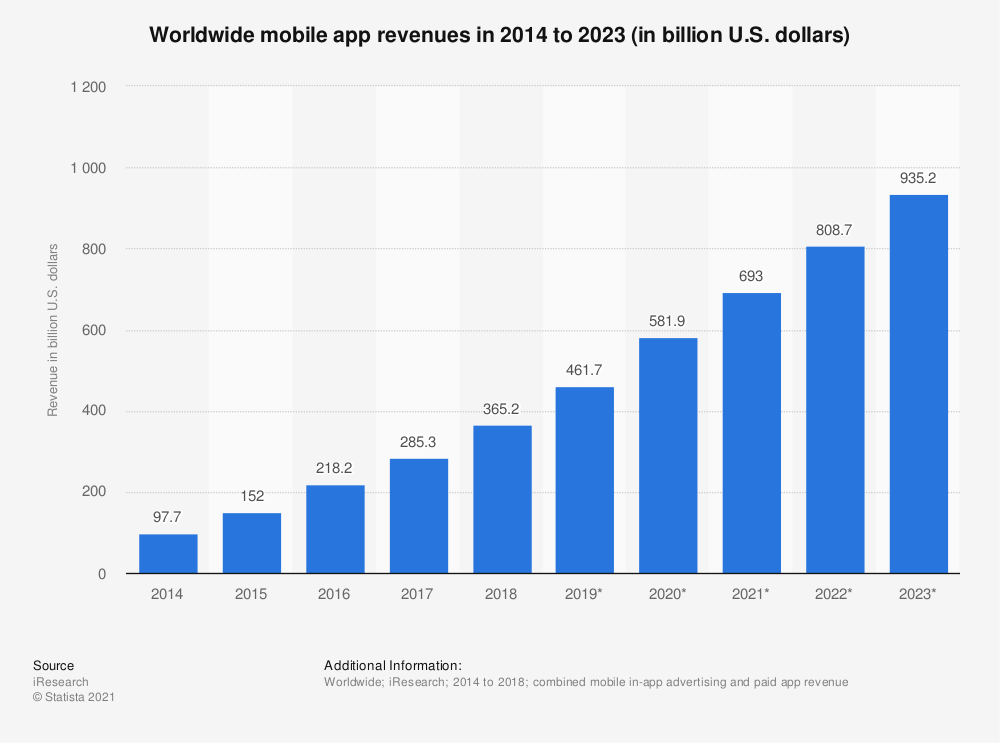
\includegraphics[scale=0.38]{kepek/mobil/total_global_mobile_app_revenues_2014-2023.png}
			\caption{A mobil alkalmazások bevétele 2014 és 2023 között világszerte}
			\label{fig:mobil:total_global_mobile_app_revenues_2014-2023}
		\end{figure}
		
		Egy 2021-ben publikált statisztikája alapján pedig megfigyelhető a Statistán, hogy 2016 és 2020 között hogyan változott a mobilos alkalmazások letöltésének száma, az egész világot beleértve (lásd: \myref{fig:mobil:annual_number_of_global_mobile_app_downloads_2016-2020} ábra).
		% TODO irodalomjegyzékhez->
		% https://www.statista.com/statistics/271644/worldwide-free-and-paid-mobile-app-store-downloads/
		\begin{figure}[h!]
			\centering
			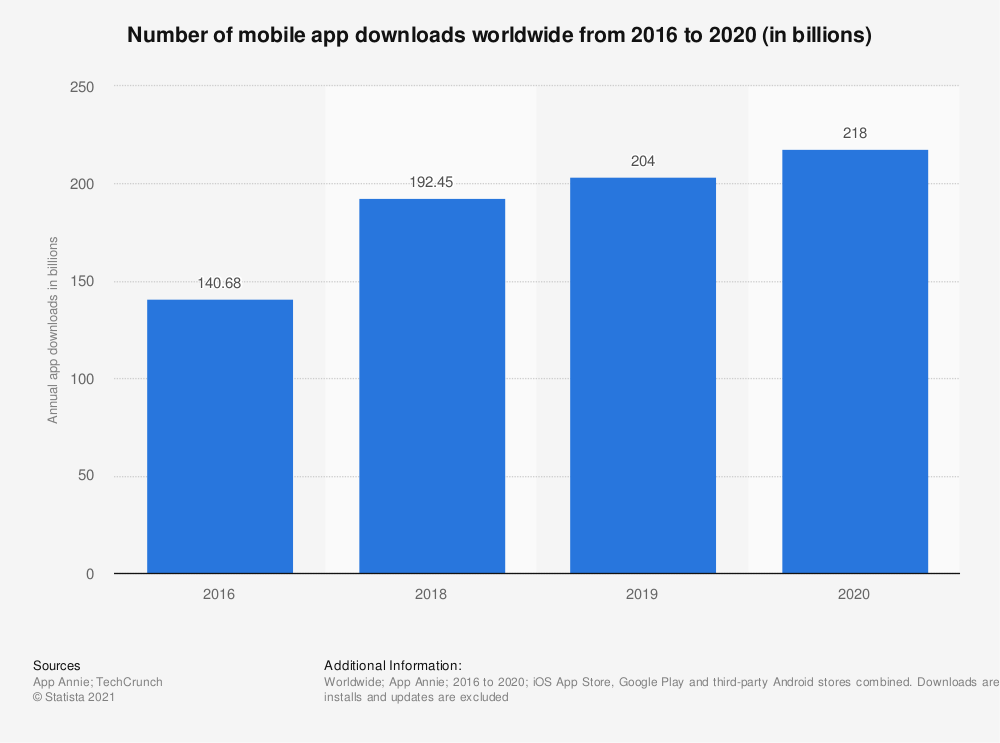
\includegraphics[scale=0.40]{kepek/mobil/annual_number_of_global_mobile_app_downloads_2016-2020.png}
			\caption{2016 és 2020 közötti mobilos alkalmazás letöltések száma világszerte}
			\label{fig:mobil:annual_number_of_global_mobile_app_downloads_2016-2020}
		\end{figure}
	
		Itt csak a legelső letöltésekre értendő az érték, az újratelepítéseket, valamint a frissítéseket már nem tartalmazzák ezek a számok. Ezenkívül megemlítendő még, hogy nem csak a két legnagyobb letöltésszámú alkalmazásbolt (azaz az iOS App Store és a Google Play), hanem az egyéb Android boltok is részt vesznek a statisztikában, mind a fizetős, mind pedig az ingyenesen letölthető alkalmazásaikkal. Közel 80 billiós emelkedést figyelhetünk meg az értékeken 2020-ra, a 2016-os 140,7 billió letöltésszámhoz képest.
		
		Ezenkívül megfigyelhetjük nem csak általánosságban a mobil applikációk, vagy a mobilos játékok bevételét, hanem összességében a játékokét is a különféle platformokon, illetve még néhány fontosabb mérföldkövet a mobilok világában (lásd: \myref{fig:mobil:Rise_of_Mobile_Gaming_Visualized} ábra).
		\begin{figure}[h!]
			\centering
			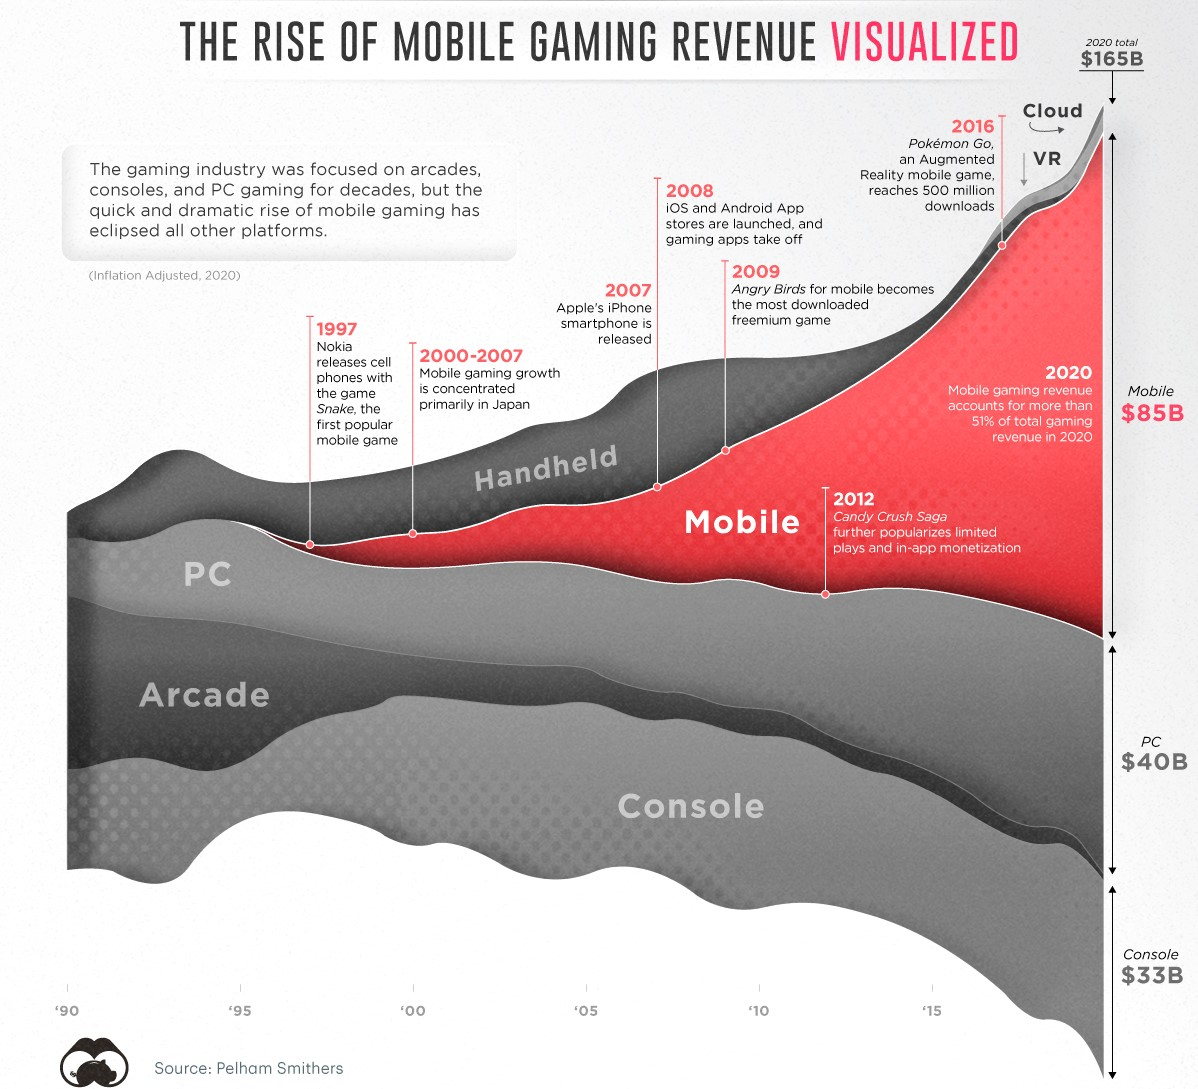
\includegraphics[scale=0.34]{kepek/mobil/Rise_of_Mobile_Gaming_Visualized.jpg}
			\caption{Mobil játékok elterjedése 1997-2020}
			\label{fig:mobil:Rise_of_Mobile_Gaming_Visualized}
		\end{figure}
		% TODO irodalomjegyzékhez->
		% https://www.visualcapitalist.com/how-big-is-the-global-mobile-gaming-industry/
		
		Az illusztráción jól látható a tendencia: a mobil platformok egyre nagyobb részét hódítják el az iparágnak. Ezért mindenképp érdemes lehet elgondolkodni, hogy egy leendő játékot milyen platformon készítünk el. Ha nem is elsődlegesen mobilra készül a játék, akkor is érdemes lehet valamilyen változatban (lebutítva, vagy más mechanikákkal kiegészítve) mobilra is kiadni azt.
		Jó példa lehetne erre a Fallout Shelter 2015-ből, amely a kezdetektől fogva mobilra is készült, vagy a League of Legends, ami eredetileg PC-re lett kiadva, azonban nemrég (2020 októberében) elkészült egy mobilos változata is, feltehetően pontosan azért, hogy a platform hatalmas játékosbázisát felhasználva még több emberhez juttassák el a játékot, és hogy ne csak a számítógép előtt ülve, de akár utazás közben is könnyedén játszhassanak a felhasználók, a gyártók pedig ezzel még több profitra tegyenek szert.

		% egyéb lehetőségek mobillal: képernyő megosztása tv-re
		A mai okostelefonokkal azonban rengeteg egyéb lehetőségünk is adódik, melyek közül párat meg is említenék, a játékokhoz kapcsolódóan. A különböző platformok, illetve a gyártók közötti határokon megfigyelhetjük, hogy már kevésbé különülnek el egymástól.
		Manapság már egyszerre konzolt és telefont is használhatnak a felhasználók egyes játékok, platformok irányításához. Például bizonyos mobilos játékokat ma már módunkban áll PlayStation kontrollerrel vezérelni. Másik hasonló lehetőség napjainkban, hogy maga az okostelefon is használható vezérlőként TV-hez és számítógéphez egyaránt, vagy akár billentyűzetet is alkalmazhatunk konzolok irányításához.
		
		Megfigyelhető, hogy egy adott játék sok esetben több különféle platformon is elérhető. A mobilos felhasználók körében igény mutakozhat arra, hogy egy konzol illetve PC játék elérhető legyen mobilon is, de fordított esetben már kevésbé merül fel ilyen igény. Például egy mobil játékot nem feltétlenül szeretne a felhasználó számítógépen játszani, hiszen a mobil könnyebben hozzáférhető, szinte mindig nálunk van, utazás közben is egyszerűen használhatjuk, játszhatunk rajta, míg a konzolokről és a PC-kről ez nem mondható el. Viszont ha mégis nagyobb képernyőn szeretnénk látni a mobilos játékot, ezt is könnyedén elérhetjük. Mostanság szinte minden háztartásban van TV készülék, és a mai technológiának köszönhetően a TV-nken is tudunk például Android játékokkal játszani, ezenkívül egyszerűen kivetíthető a telefon képernyője TV-re (vagy épp PC-re), így játszhatunk az eszközön telefonos játékokkal is.
		% TODO irodalomjegyzék->
		% https://gadget-info.com/66728-15-best-android-tv-games-you-should-play
		% https://www.origo.hu/techbazis/20150826-android-tv-sony-bravia-4k-google-operacios-rendszer-alkalmazasok-uj-orulet.html
		% https://www.cnet.com/how-to/unified-remote-turns-your-android-into-a-pc-controller/
		% TODO 	-sokan: mobil app-nak álcáznak weboldalakat (ma már számos- html5 js ts) de valójában html alapú, csak egy app-ba van becsomagolva <- ezekről pár oldal	(ionic, react native, etc) js-es alkalmazást weben/androidon ios-en akár windowson is futtathatóvá teszi PL discord
		\end{MySubSection}

		% ->végül nem ide lesz írva -webes(általánosan, később részletezve)		
		% TODO 	-hardveres gyorsítós böngészős játékok
		% TODO 	-elérhető technológiák / irányok
		% TODO 	-Jövő: a javascript mert az futtatható mindenhol (ha nem túl erőforrás igényes az alkalmazás)
	\end{MySection}

	\begin{MySection}{Játékfejlesztés keretrendszerek nélkül}
		% c++, low-level 
		Keretrendszerek nélküli fejlesztés esetén rendszerint inkább alacsonyabb szintű programozási nyelveken fejlesztenek, mint pédéul a C++, mert általában eleve a sebesség miatt nem alkalmaznak keretrendszert, ezért feltehetően olyan programozási nyelvet használnak mellé, ami elősegíti azt, hogy gyorsan futó kódot tudjunk írni.
		
		% előny
		A keretrendszerek nélküli játékfejlesztésnek a sebességen kívül is számos előnye lehet a használatukkal szemben, főleg tapasztaltabb fejlesztők számára, többek között:
		\begin{itemize}
			\item Itt mindent saját magának készít el a fejlesztő, ezért ez a fejlesztési módszer kevésbé kötött, nagyobb rugalmasságot ad.
			\item Egy idő után, ha sokat fejlesztünk játékmotorok használata nélkül, kialakul egy általunk fejlesztett "keretrendszer". Ez persze nem biztos, hogy valóban egy komplett játékmotor, viszont azon amit tartalmaz könnyedén kiigazodhatunk, mert egyből tudjuk, mit hol kell keresnünk a kódban.
			\item Főleg az előző ok miatt, ha hibát ejtünk valahol, könnyebb kijavítani.
		\end{itemize}
	
		% hátrány
		Kezdő, tapasztalatlanabb játékfejlesztők számára azonban hátrány lehet, hogy ez a folyamat sokkal lassabb, időigényesebb lehet, mint egy már meglévő motor használatával elkészített alkalmazás.

		% TODO 	- példa ilyenre
	\end{MySection}

	\begin{MySection}{Játékfejlesztés keretrendszerekkel}
		% game-engine mit tartalmaz
		A keretrendszerek, azaz a grafikus motorok és a játékmotorok használata a 2000 körüli években vált kimondottan gyakorivá, nagy lökést kaptak a grafikus processzorok megjelenése után.
		
		A grafikus-, valamint a játékmotorokat céljainktól függően fontos megkülönböztetnünk egymástól, ez funkcionalitásuk szerint egyszerűen kivitelezhető:
		\begin{itemize}
			\item Grafikus motorok csak képi megjelenítésben segítik a programozót.
			\item Játékmotorok ennél bővebb, egy nagyobb eszközrendszert biztosítanak a fejlesztőknek.
		\end{itemize}
		% előny
		Mivel játékfejlesztéshez egy játékmotor használata a célszerűbb, mint a grafikus motoré, ezért a fejezetben főleg a játékmotorokról lesz szó bővebben.
		A játékmotorok használata tehát előnyös lehet az effektívebb, gyorsabb játékfejlesztéshez. Mivel a számítógépes grafika magas szinten van, szükség lehet a motor komplex funkcionalitására. A technológia fejlődése által egyre szebb látványvilágot tudnak visszaadni mind a grafikus-, mind a játékmotorok. Használatukkal viszont rengeteg erőforrás megspórolható azzal, hogy nem a fejlesztő feladata megvalósítani például a fizikai alrendszert, ütközésvizsgálatot, a megjelenítésért felelős rendszert, stb.
		Nem csak az egész játékmotort egyben, hanem önmagában csak egy-egy alrendszert is lehetőségünk van megvásárolni, mely abban az esetben lehet például kifizetődő, ha egy már kipróbált, megfelelő alrendszert beszerezni olcsóbb, mint egy saját, új alrendszer kifejlesztése. \cite{mileff}
		% TODO irodalom -> 
		% https://users.iit.uni-miskolc.hu/~mileff/grafika/Grafika_programozasa_jegyzet_v0.66_Mileff_P.pdf
		A mobilok megjelenésével új terület nyílt meg a keretrendszerek számára, több ismert játékmotort forgalmazó cég hordozható eszközökre elérhető változatot is adott ki.
		Keretrendszert használhatunk számítógépre, konzolra, valamint mobil eszközre való fejlesztésre egyaránt, a célplatformtól függően számos motor közül válogathatunk. Létezik külön 2D-s valamint 3D-s alkalmazás fejlesztéséhez megfelelő játékmotor, illetve van, amelyik mindkettőre alkalmas.
		
		% hátrány
		A fentebb említett főbb előnyei miatt, egy modern motor vásárlása nagy költséget jelenthet a fejlesztők számára, ami nem meglepő, mert nagyon sok munka van az elkészítésében.
		Az esetlegesen magas áron felül, hátránya lehet még, hogy a fejlesztésben kevesebb rugalmasság, szabadság van, illetve nehezebb kijavítani az esetleges hibákat fejlesztés közben.
		
		% TODO 	- opengl
		% Megemlítendő az OpenGL, mert ez az egyik legrégebbi, tulajdonképpen azért fontos megemlíteni mert egy alap motor.
		%- open-source, - platformfüggetlen, bármilyen oprendszeren működik az opengl-es alkalmazás, leginkább a videokártya határozza meg h milyen funkciókat lehet vele használni. 
		% opengl bonyolult használat, kevésbé népszerű, már jobb és gyorsabb megoldások is vannak
		% nem feltétlenül szokták játékfejlesztéshez használni, mert bonyolultabb dolgokat nehéz benne összerakni, de egyszerűbb játékokhoz, vagy akár csak szemléltetéshez példákhoz ezt is lehet használni.
		% már van modernebb verziója is, aminek már jobb a teljesítménye, de még továbbra sem terjedt el eléggé ahhoz, hogy nagyobb projekthez érdemes legyen számításba venni.		-> még ha ugyan olyan jó is lenne mint a többi, mivel kevesen használják, ha problémába ütközöl feltehetően magadtól kell megoldanod, mert nem feltétlenül találsz rá megoldást az interneten
		
		\begin{MySubSection}{Mai ismertebb keretrendszerek}
		% game-engine-k
		Napjainkban számos játékfejlesztésre (és egyéb alkalmazások fejlesztésére) alkalmas keretrendszer megtalálható a piacon, mint már szó volt róla, több platform terén is.
		\newline \newline
		Ezek közül példaként néhány közkedvelt:
		\begin{itemize}
			\item CryEngine
			\item Unity
			\item Unreal Engine
			\item Source
		\end{itemize}
		Természetesen ennél sokkal több játékmotor létezik, melyeket az interneten könnyedén megtalálhatunk, és néhányat akár ingyenesen is letölthetünk.
		Például a következő linken: \url{https://en.wikipedia.org/wiki/List\_of\_game\_engines} találhatunk a Wikipédián egy listát rengeteg keretrendszerről (a teljesség igénye nélkül), ahol a nevüket, az elsődleges programozási nyelvüket, a célplatformjukat, az adott játékmotor közreműködésével elkészült játékok listáját, valamint egyéb tényezőket is megtekinthetünk.
		\end{MySubSection}
		% TODO 	- unity
		
		\begin{MySubSection}{Unreal Engine}
		% unreal engine
		Vegyük példának az egyik népszerű, modern játékmotorra az Unreal Enginet. A motort 1995-ben kezdte el írni az Epic Games (amerikai játék-, illetve szoftverfejlesztő és kiadó cég) alapítója, név szerint Tim Sweeney. Eredetileg azzal a céllal, hogy elősegítse egy játék fejlesztési folyamatát, amely Unreal névvel jelent meg, több év után, 1998-ban. Az Unreal nevű játék egy First-Person Shooter (röviden: FPS, ez a műfaj magyarul belső nézetű lövöldözős játékot jelent), kezdetben tehát a motor FPS játékok fejlesztéséhez íródott. Azóta viszont rengeteget fejlődött, és már számos népszerű játék készült el a segítségével, nem csak FPS, hanem egyéb kategóriákban is, például MMORPG (azaz a már korábban említett többszereplős online szerepjátékműfaj), vagy platformer játékok (ide sorolható minden olyan játék, melynek nagy részét képezi a platformokon való ugrálás). A keretrendszer fejlődésén jelenleg is dolgoznak, a következő verziójából, az Unreal Engine 5-ből már nyilvánosságra is hoztak egy kis ízelítőt, a teljes verziót pedig a 2021-es év végére tervezik kiadni.
		% TODO irodalom ->
		% https://en.wikipedia.org/wiki/Unreal_Engine
		% https://www.unrealengine.com/en-US/blog/a-first-look-at-unreal-engine-5
		% https://en.wikipedia.org/wiki/Epic_Games
		% https://hu.wikipedia.org/wiki/First-person_shooter
		% https://www.google.com/search?tbm=bks&q=isbn:9780429560576
		
		% példák
		A fejlődés szemléltetéseként mellékelek egy-egy fotót a motor régebbi verziójával készült, 2001-ben PlayStationre kiadott Harry Potter és a bölcsek köve játékról (lásd: \myref{fig:unrealEngine:harry-potter-and-the-sorcerer-s-stone-ps} ábra), valamint az Unreal Engine 5 által készített PlayStation 5-ön futó demóról, mely 2020-ban látott napvilágot (lásd: \myref{fig:unrealEngine:First-look-at-Unreal_Engine_5} ábra). A platform tehát mindkét esetben konzol volt, viszont a technológia fejlődése kifejezetten szembetűnő, a 2001-es, illetve a majdnem 20 évvel későbbi fénykép között.
		\begin{figure}[h!]
			\centering
			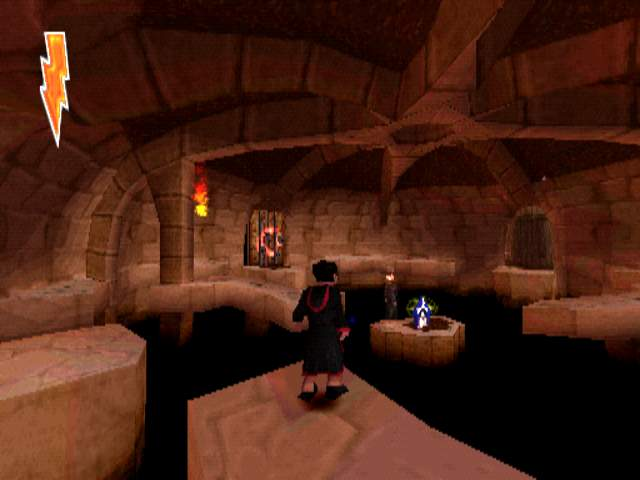
\includegraphics[scale=0.4]{kepek/unrealEngine/harry-potter-and-the-sorcerer-s-stone-ps.jpeg}
			\caption{Harry Potter és a bölcsek köve PlayStation játék (2001)}
			\label{fig:unrealEngine:harry-potter-and-the-sorcerer-s-stone-ps}
		\end{figure}
		\begin{figure}[h!]
			\centering
			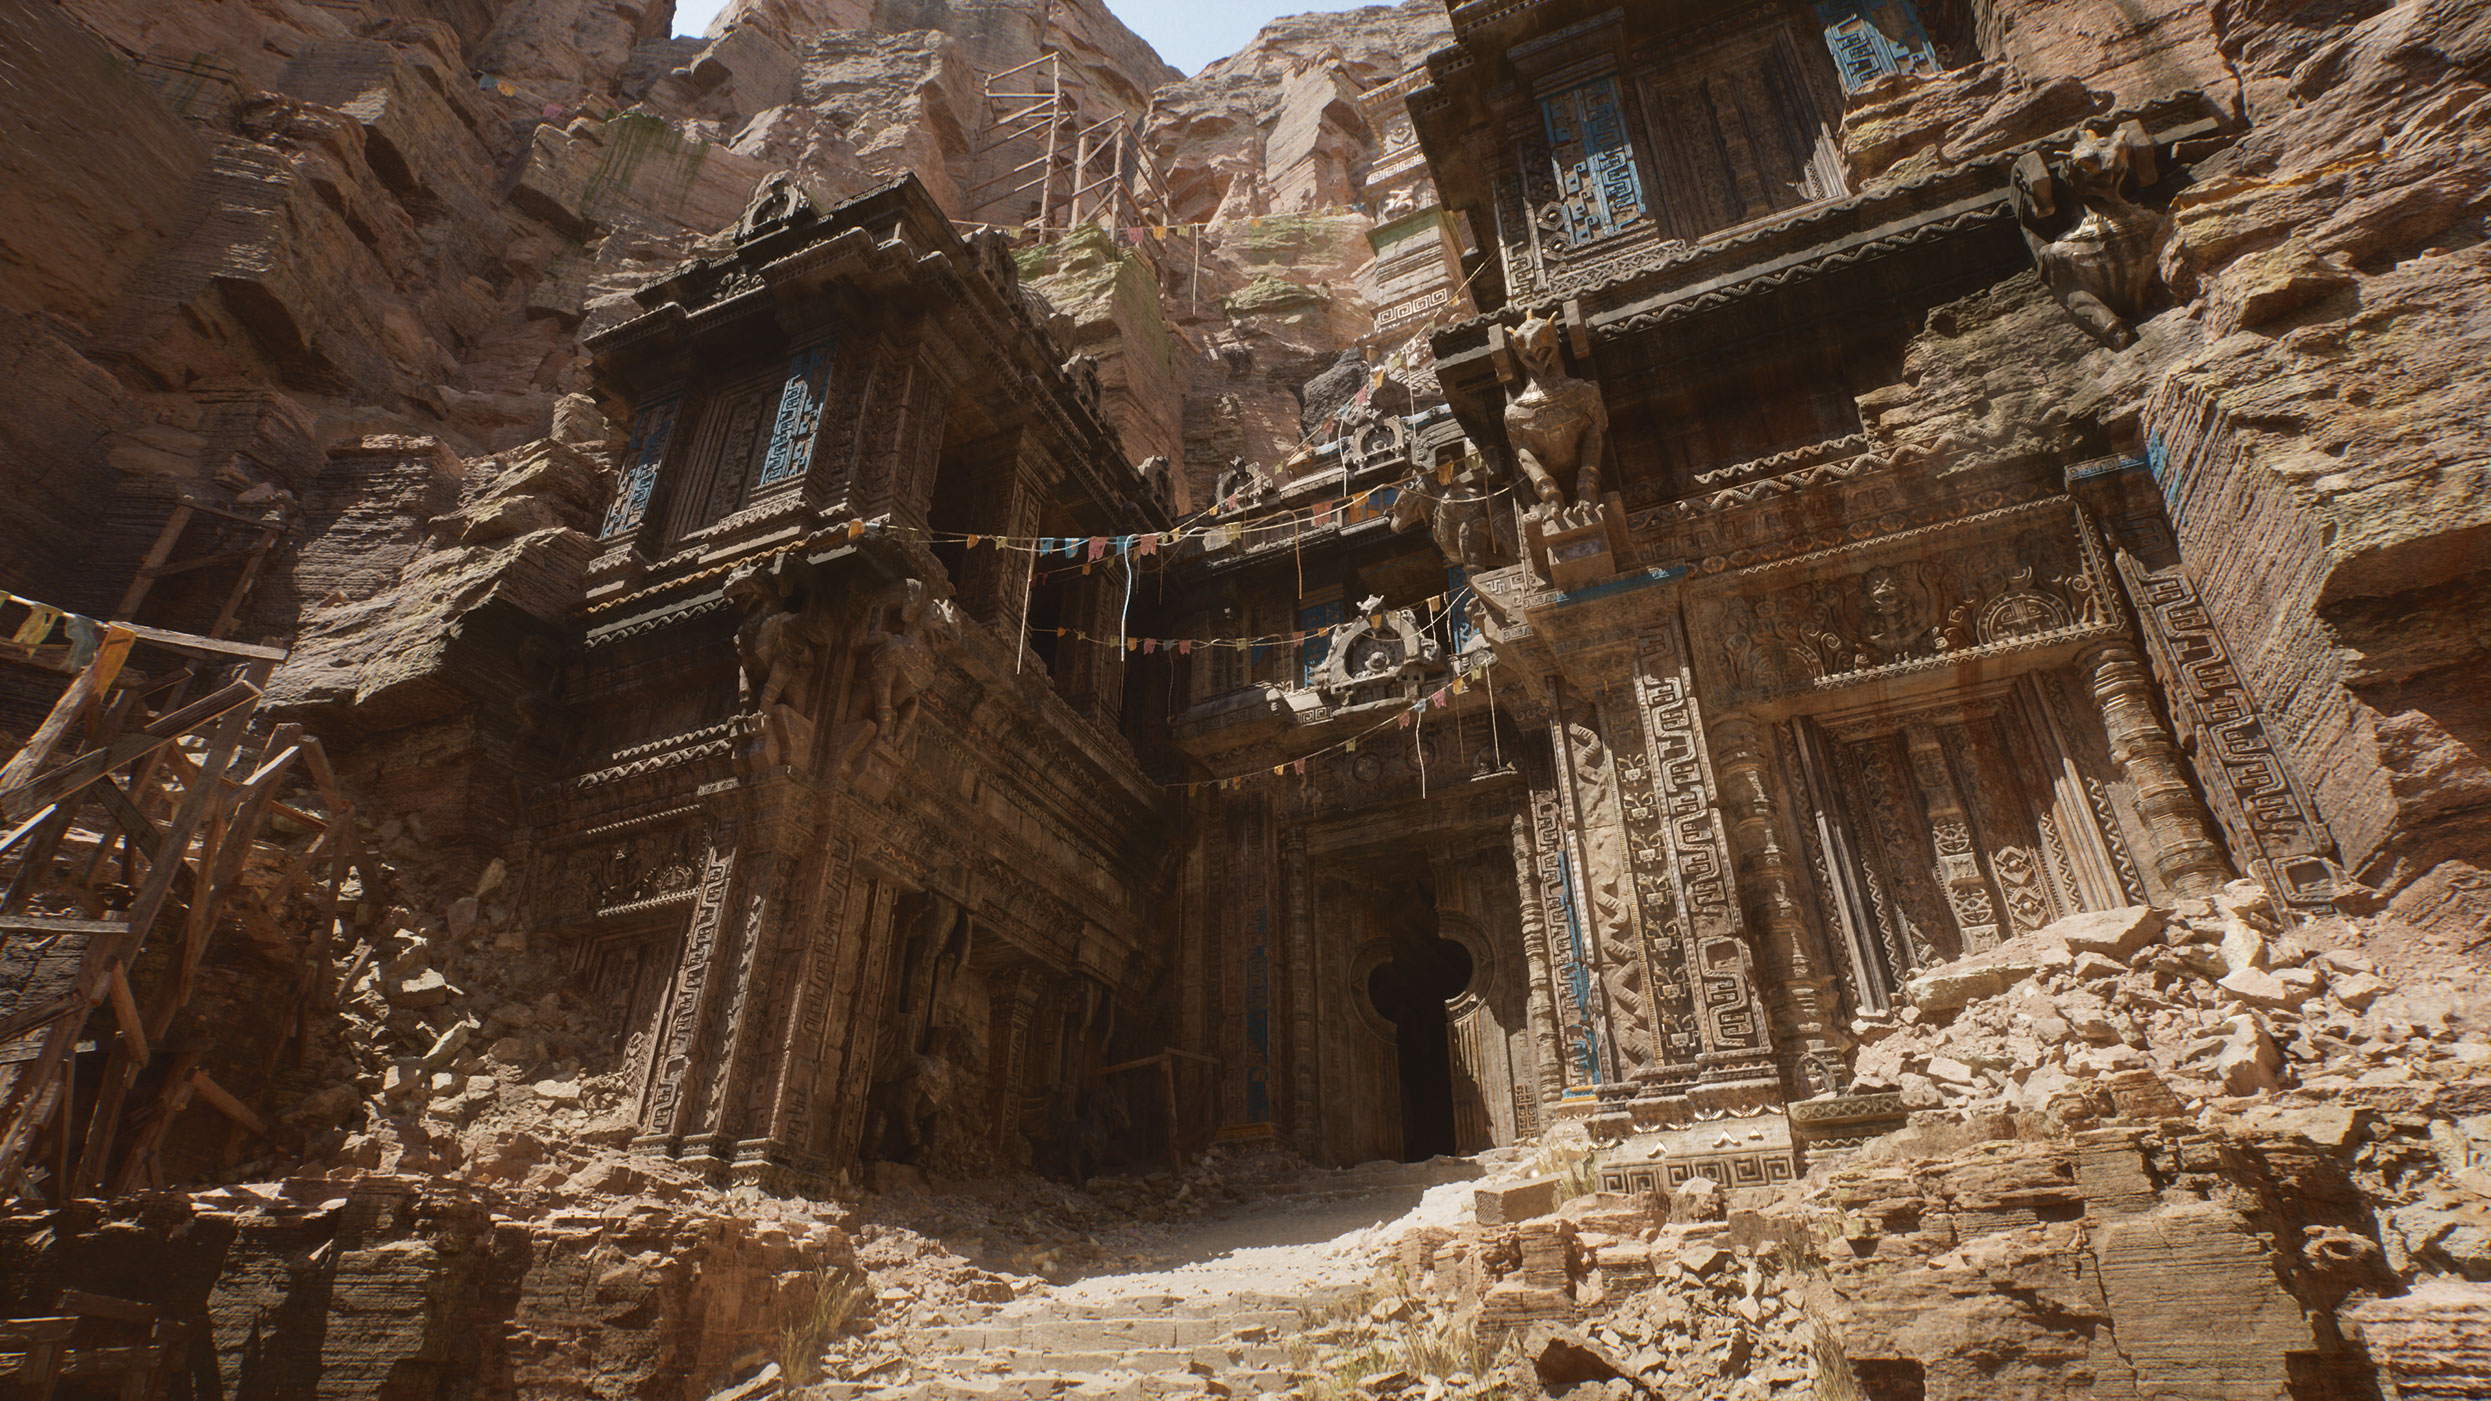
\includegraphics[scale=0.16]{kepek/unrealEngine/First-look-at-Unreal_Engine_5.jpg}
			\caption{Unreal Engine 5 demó (2020)}
			\label{fig:unrealEngine:First-look-at-Unreal_Engine_5}
		\end{figure}
	
		A képeket szemügyre véve tisztán látható a különbség, hogy az újabb változata a keretrendszernek mennyivel filmszerűbb, részlegtagazdabb látványvilágot képes nyújtani.
		% TODO forrás->
		% https://tcrf.net/Prerelease:Harry_Potter_and_the_Sorcerer%27s_Stone_(PlayStation)
		% https://www.unrealengine.com/en-US/blog/a-first-look-at-unreal-engine-5
		\end{MySubSection}
		
		% TODO 	- telepítésük
		% TODO 	- használatuk
		% TODO 	- tapasztalatok (kipróbálás ha lehet)
		% TODO 	(- összehasonlítás, konklúzió)
		% TODO - táblázatos formában összehasonlítás esetleg?
		
		% TODO 	- statisztikák, kezelhetőség, tanulhatóság, gyorsaság stb
		\end{MySection}
	
\end{MyChapter}
		
% TODO használt linkek hozzáadása az irodalomjegyzékhez
% https://en.wikipedia.org/wiki/Video_game_development
% https://en.wikipedia.org/wiki/Steve_Russell_(computer_scientist) / VAGY / https://www.computerhistory.org/pdp-1/steve-slug-russell/
% https://www.theverge.com/2013/2/4/3949524/the-story-of-the-worlds-first-digital-video-game
% https://en.wikipedia.org/wiki/PC_game
% https://en.wikipedia.org/wiki/History_of_video_games
% https://en.wikipedia.org/wiki/OXO
% https://en.wikipedia.org/wiki/Colossal_Cave_Adventure
% https://hu.wikipedia.org/wiki/Tennis_for_Two

% https://techcrunch.com/2015/10/31/the-history-of-gaming-an-evolving-community/

% https://www.gamedesigning.org/gaming/history/
% https://www.lifewire.com/magnavox-odyssey-the-first-gaming-console-729587
% https://hu.wikipedia.org/wiki/Pong
% https://www.history.com/topics/inventions/history-of-video-games
% https://en.wikipedia.org/wiki/Activision
% https://www.activision.com/company/aboutus

% https://mediag.com/blog/reality-bytes-cautious-optimism-and-the-video-game-crash-of-1983/
% https://hu.wikipedia.org/wiki/Nintendo
% https://hu.wikipedia.org/wiki/Game_Boy
% https://hu.wikipedia.org/wiki/PlayStation_(konzol)
% https://hu.wikipedia.org/wiki/Vide%C3%B3j%C3%A1t%C3%A9k-konzol

% https://www.techspot.com/article/650-history-of-the-gpu/
% https://www.techspot.com/article/653-history-of-the-gpu-part-2/
% https://hu.wikipedia.org/wiki/ATI_Technologies
% https://hu.wikipedia.org/wiki/Nvidia

% https://hu.wikipedia.org/wiki/MMORPG
